\documentclass[12pt,letterpaper]{article}
\usepackage{graphicx,textcomp}
\usepackage{natbib}
\usepackage{setspace}
\usepackage{fullpage}
\usepackage{color}
\usepackage[reqno]{amsmath}
\usepackage{amsthm}
\usepackage{fancyvrb}
\usepackage{amssymb,enumerate}
\usepackage[all]{xy}
\usepackage{endnotes}
\usepackage{lscape}
\newtheorem{com}{Comment}
\usepackage{float}
\usepackage{hyperref}
\newtheorem{lem} {Lemma}
\newtheorem{prop}{Proposition}
\newtheorem{thm}{Theorem}
\newtheorem{defn}{Definition}
\newtheorem{cor}{Corollary}
\newtheorem{obs}{Observation}
\usepackage[compact]{titlesec}
\usepackage{dcolumn}
\usepackage{tikz}
\usetikzlibrary{arrows}
\usepackage{multirow}
\usepackage{xcolor}
\newcolumntype{.}{D{.}{.}{-1}}
\newcolumntype{d}[1]{D{.}{.}{#1}}
\definecolor{light-gray}{gray}{0.65}
\usepackage{url}
\usepackage{listings}
\usepackage{color}

\definecolor{codegreen}{rgb}{0,0.6,0}
\definecolor{codegray}{rgb}{0.5,0.5,0.5}
\definecolor{codepurple}{rgb}{0.58,0,0.82}
\definecolor{backcolour}{rgb}{0.95,0.95,0.92}

\lstdefinestyle{mystyle}{
	backgroundcolor=\color{backcolour},   
	commentstyle=\color{codegreen},
	keywordstyle=\color{magenta},
	numberstyle=\tiny\color{codegray},
	stringstyle=\color{codepurple},
	basicstyle=\footnotesize,
	breakatwhitespace=false,         
	breaklines=true,                 
	captionpos=b,                    
	keepspaces=true,                 
	numbers=left,                    
	numbersep=5pt,                  
	showspaces=false,                
	showstringspaces=false,
	showtabs=false,                  
	tabsize=2
}
\lstset{style=mystyle}
\newcommand{\Sref}[1]{Section~\ref{#1}}
\newtheorem{hyp}{Hypothesis}

\title{Problem Set 1}
\date{Due: October 3, 2021}
\author{Applied Stats/Quant Methods 1}

\begin{document}
	\maketitle
	
	\section*{Linette Lim}
	\vspace{.7cm}
	\section*{Question 1 (50 points): Education}

A school counselor was curious about the average of IQ of the students in her school and took a random sample of 25 students' IQ scores. The following is the data set:\\
\vspace{.5cm}

\lstinputlisting[language=R, firstline=5, lastline=5]{PS1_answers_LL.R}  

\vspace{.5cm}

\begin{enumerate}
	\item Find a 90\% confidence interval for the average student IQ in the school.\\
	
	\item Next, the school counselor was curious  whether  the average student IQ in her school is higher than the average IQ score (100) among all the schools in the country.\\ 
	
	\noindent Using the same sample, conduct the appropriate hypothesis test with $\alpha=0.05$.
\end{enumerate}

\begin{itemize}	
\item
Answer for Question 1.1\\
\noindent First, load packages such as Tidyverse and set the working directory.\\ 
\noindent Assign the dataset of 25 students’ IQ scores to an object, "y".\\
\noindent Next, check the data using functions like summary(), mean(), sd(). We get:\\
\begin{verbatim}
> summary(y)
   Min. 1st Qu.  Median    Mean 3rd Qu.    Max. 
  69.00   89.00   98.00   98.44  110.00  126.00 
> sd <- sd(y)
> sd
[1] 13.09287
> y.bar <- mean(y)
> y.bar
[1] 98.44
> se <- sd(y)/sqrt(length(y)) 
> se
[1] 2.618575
\end{verbatim}
\vspace{.3cm}
\noindent Check the distribution of the data and calculate the lower and upper ends of the 90 percent confidence interval using qnorm():\\
\vspace{.3cm}
\lstinputlisting[language=R, firstline=20, lastline=28]{PS1_answers_LL.R}  
\vspace{.3cm}
\noindent We get:
\begin{verbatim}
    Lower    Upper
 94.13283 102.7472
\end{verbatim}
\vspace{.3cm}
\noindent We can check this answer with t.test():\\
\vspace{.3cm}
\lstinputlisting[language=R, firstline=32, lastline=34]{PS1_answers_LL.R}  
\vspace{.3cm}
\noindent We get:
\begin{verbatim}
	One Sample t-test

data:  y
t = 37.593, df = 24, p-value < 2.2e-16
alternative hypothesis: true mean is not equal to 0
90 percent confidence interval:
  93.95993 102.92007
sample estimates:
mean of x 
    98.44
\end{verbatim}
\vspace{.3cm}
\noindent Therefore we can conclude that with 90 percent confidence, the average student IQ in the school is between 94 and 103.\\
\end{itemize}

\begin{itemize}	
\item
Answer for Question 1.2\\
\noindent We  are told the average IQ score among all the schools in the country is 100. Therefore, let mu = 100. 
\noindent The null and alternative hypotheses are formulated as follows:
\vspace{.5cm}
\lstinputlisting[language=R, firstline=43, lastline=44]{PS1_answers_LL.R}  
\vspace{.5cm}
\noindent Since the alternative hypothesis is $y.bar > 100$, we compute the one-sided p-value as follows:
\vspace{.5cm}
\lstinputlisting[language=R, firstline=46, lastline=46]{PS1_answers_LL.R}  
\vspace{.5cm}
\noindent The p-value calculated is:
\begin{verbatim}
[1] 0.7243269
\end{verbatim}
\vspace{.3cm}
\noindent We can check this answer using the z score and pnorm() formula:
\vspace{.5cm}
\lstinputlisting[language=R, firstline=51, lastline=52]{PS1_answers_LL.R}  
\vspace{.5cm}
\noindent We get the same answer. The p-value is 0.7243269. This is larger than the significance level alpha = 0.05, so we cannot reject the null hypothesis. There is not enough statistical evidence to support Ha, that is, that the average IQ in the school is higher than the average IQ score (100) among all the schools in the country.

\newpage

	\section*{Question 2 (50 points): Political Economy}

\noindent Researchers are curious about what affects the amount of money communities spend on addressing homelessness. The following variables constitute our data set about social welfare expenditures in the USA. \\
\vspace{.5cm}


\begin{tabular}{r|l}
	\texttt{State} &\emph{50 states in US} \\
	\texttt{Y} & \emph{per capita expenditure on shelters/housing assistance in state}\\
	\texttt{X1} &\emph{per capita personal income in state} \\
	\texttt{X2} &  \emph{Number of residents per 100,000 that are "financially insecure" in state}\\
	\texttt{X3} &  \emph{Number of people per thousand residing in urban areas in state} \\
	\texttt{Region} &  \emph{1=Northeast, 2= North Central, 3= South, 4=West} \\
\end{tabular}

\vspace{.5cm}
\noindent Explore the \texttt{expenditure} data set and import data into \texttt{R}.
\vspace{.5cm}
\lstinputlisting[language=R, firstline=54, lastline=54]{PS01.R}  
\vspace{.5cm}
\begin{itemize}

\item
Please plot the relationships among \emph{Y}, \emph{X1}, \emph{X2}, and \emph{X3}? What are the correlations among them (you just need to describe the graph and the relationships among them)?
\vspace{.5cm}

\item
Please plot the relationship between \emph{Y} and \emph{Region}? On average, which region has the highest per capita expenditure on housing assistance?
\vspace{.5cm}
\item
Please plot the relationship between \emph{Y} and \emph{X1}? Describe this graph and the relationship. Reproduce the above graph including one more variable \emph{Region} and display different regions with different types of symbols and colors.
\end{itemize}

\item
Answer for Question 2.1\\

\noindent First we import the data:\\
\vspace{.5cm}
\lstinputlisting[language=R, firstline=69, lastline=69]{PS1_answers_LL.R}  
\vspace{.5cm}

\noindent Next, we plot each pair of variables and generate 12 graphs using the following formula:\\
\vspace{.5cm}
\lstinputlisting[language=R, firstline=72, lastline=74]{PS1_answers_LL.R}  
\vspace{.5cm}

\noindent We plot the 12 graphs (see Figures 1 - 12 from page 7 to page 18) to examine the correlations, using Y, followed by X1, then X2, and finally X3, as the response variable.\\

\noindent Fig 1 shows a weak, positive, linear relationship between Y, per capita expenditure on shelters/housing assistance in state, and X1, the per capita personal income in state. There are a number of outliers in the data that need to be investigated.\\

\noindent Fig 2 shows a weak, positive, linear relationship between Y, per capita expenditure on shelters/housing assistance in state, and X2, the number of residents per 100,000 that are ”financially insecure” in state. There are a number of outliers in the data that need to be investigated.\\

\noindent Fig 3 shows a moderately strong, positive, linear relationship between Y, per capita expenditure on shelters/housing assistance in state, and X3, the number of people per thousand residing in urban areas in state. This suggests it is likely that the greater the number of urban residents in state, the greater the expenditure on shelters/housing assistance in state. There are a few outliers in the data.\\ 

\noindent Fig 4 shows a weak, positive, linear relationship between Y, per capita expenditure on shelters/housing assistance in state, and X1, the per capita personal income in state. There are a number of outliers in the data that needs to be investigated.\\

\noindent Fig 5. The points on the scatter plot seem to be scattered randomly, suggesting that there is no relationship or no correlation between X2, the number of residents per 100,000 that are ”financially insecure” in state, and X1, the per capita personal income in state.\\

\noindent Fig 6 shows a moderately strong, positive, linear association between X3, the number of people per thousand residing in urban areas in state, and X1, the per capita personal income in state. This suggests it is likely that the greater the number of people living in urban areas in state, the greater the per capita personal income in state. There are a few outliers that need to be investigated.\\

\noindent Fig 7 shows a weak, positive, linear relationship between Y, per capita expenditure on shelters/housing assistance in state, and X2, the number of residents per 100,000 that are ”financially insecure” in state. There are a number of outliers in the data that need to be investigated.\\

\noindent Fig 8. The points on the scatter plot seem to be scattered randomly, suggesting that there is no relationship or no correlation between X1, the per capita personal income in state, and X2, the number of residents per 100,000 that are ”financially insecure” in state.\\

\noindent Fig 9. The points on the scatter plot seem to be scattered randomly, suggesting there is no relationship or no correlation between X3, the number of people per thousand residing in urban areas in state, and X2, the number of residents per 100,000 that are ”financially insecure” in state.\\

\noindent Fig 10 shows a weak, positive, linear relationship between Y, per capita expenditure on shelters/housing assistance in state, and X3, the number of people per thousand residing in urban areas in state. There are a number of outliers in the data.\\

\noindent Fig 11 shows a moderately strong, positive, linear association between X1, the per capita personal income in state, and X3, the number of people per thousand residing in urban areas in state. This suggests it is likely that the greater the per capita personal income in state, the greater the number of people living in urban areas in state. There are a number of outliers in the data that need to be investigated.\\

\noindent Fig 12. The points on the scatter plot seem to be scattered randomly, suggesting there is no relationship or no correlation between X2, Number of residents per 100,000 that are ”financially insecure” in state, and X3, the number of people per thousand residing in urban areas in state.\\

\newpage

Graphs for Question 2.1\\

\begin{figure}[hbtp!]\centering
	\caption{\footnotesize Relationship between Y and X1.}
	\label{fig:plot_1}
	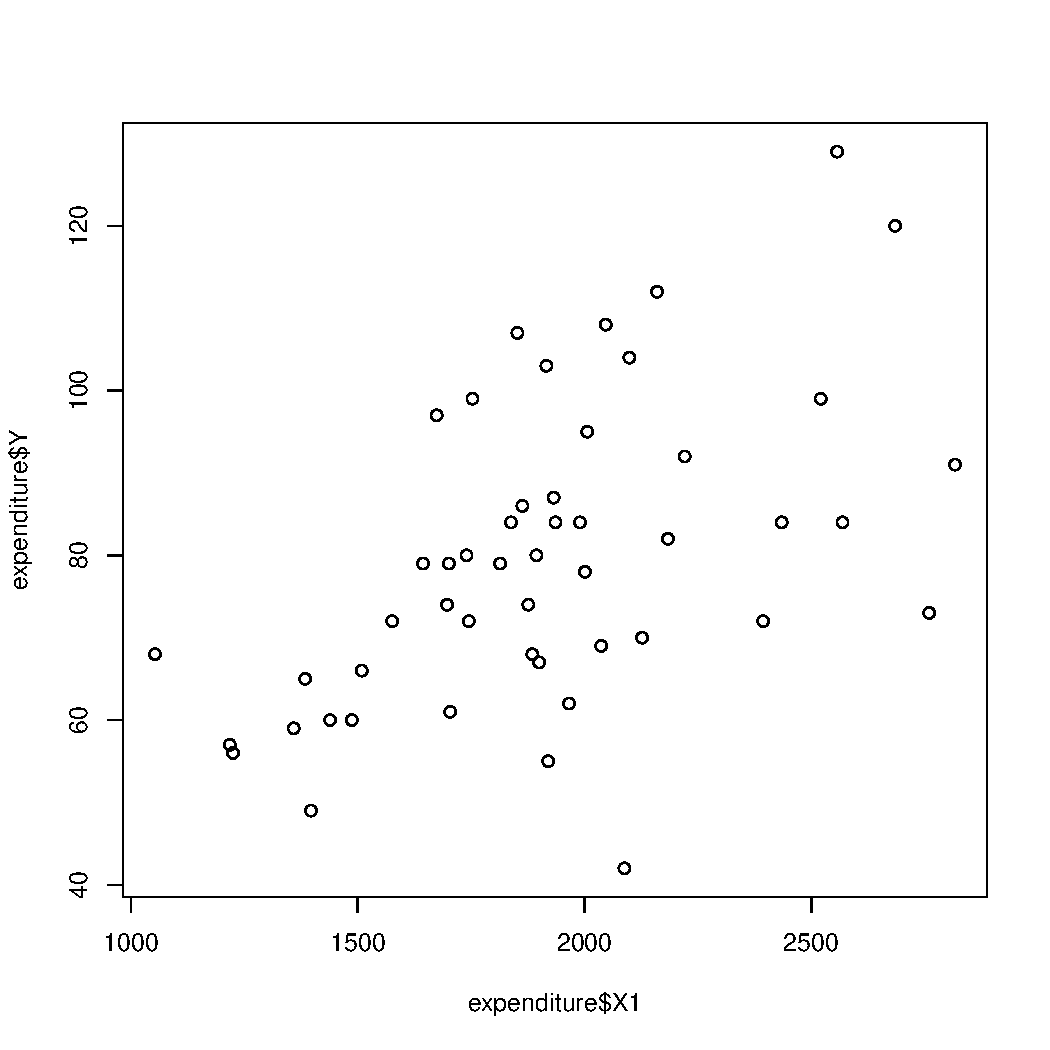
\includegraphics[width=.75\textwidth]{plot1_Y_X1.pdf}
\end{figure}

\begin{figure}[hbtp!]\centering
	\caption{\footnotesize Relationship between Y and X2.}
	\label{fig:plot_2}
	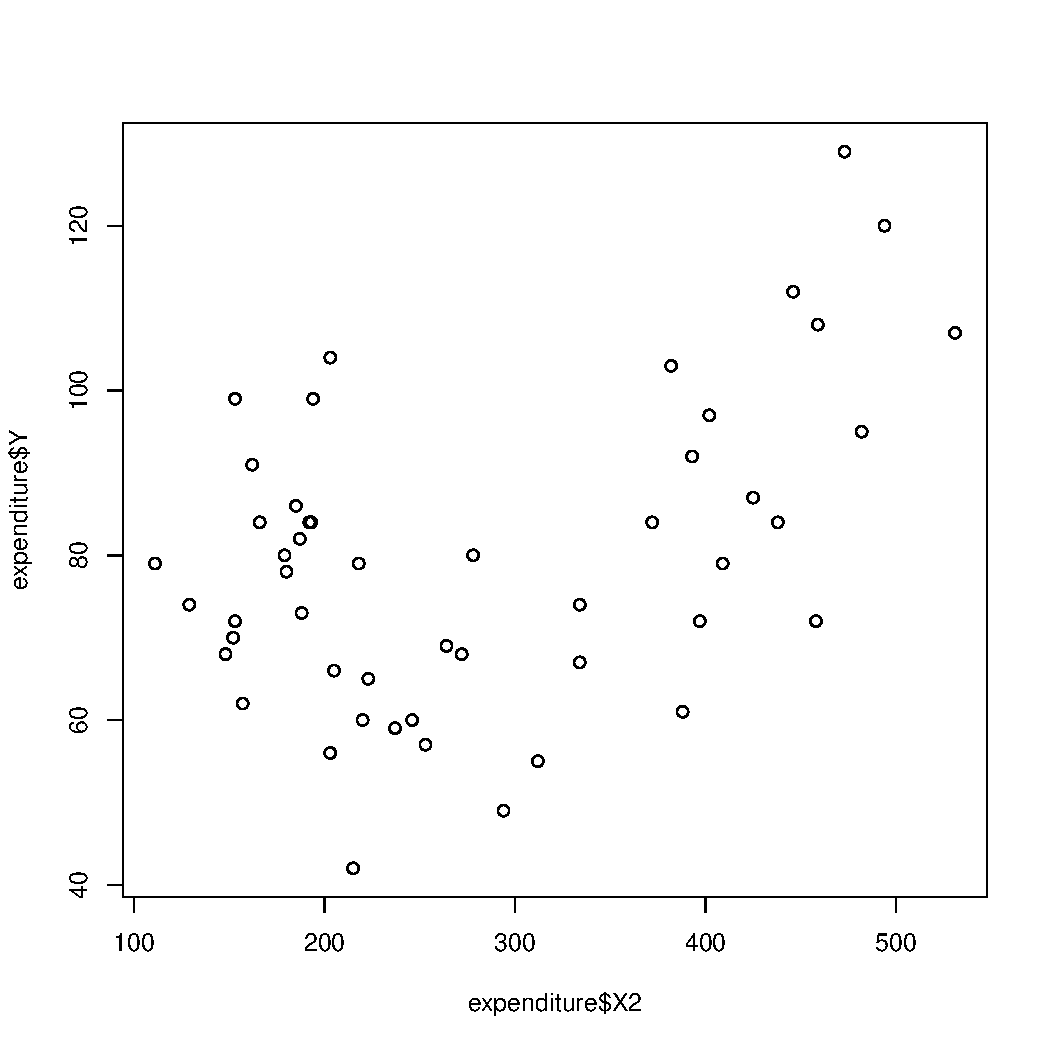
\includegraphics[width=.75\textwidth]{plot_Y_X2.pdf}
\end{figure}

\begin{figure}[hbtp!]\centering
	\caption{\footnotesize Relationship between Y and X3.}
	\label{fig:plot_3}
	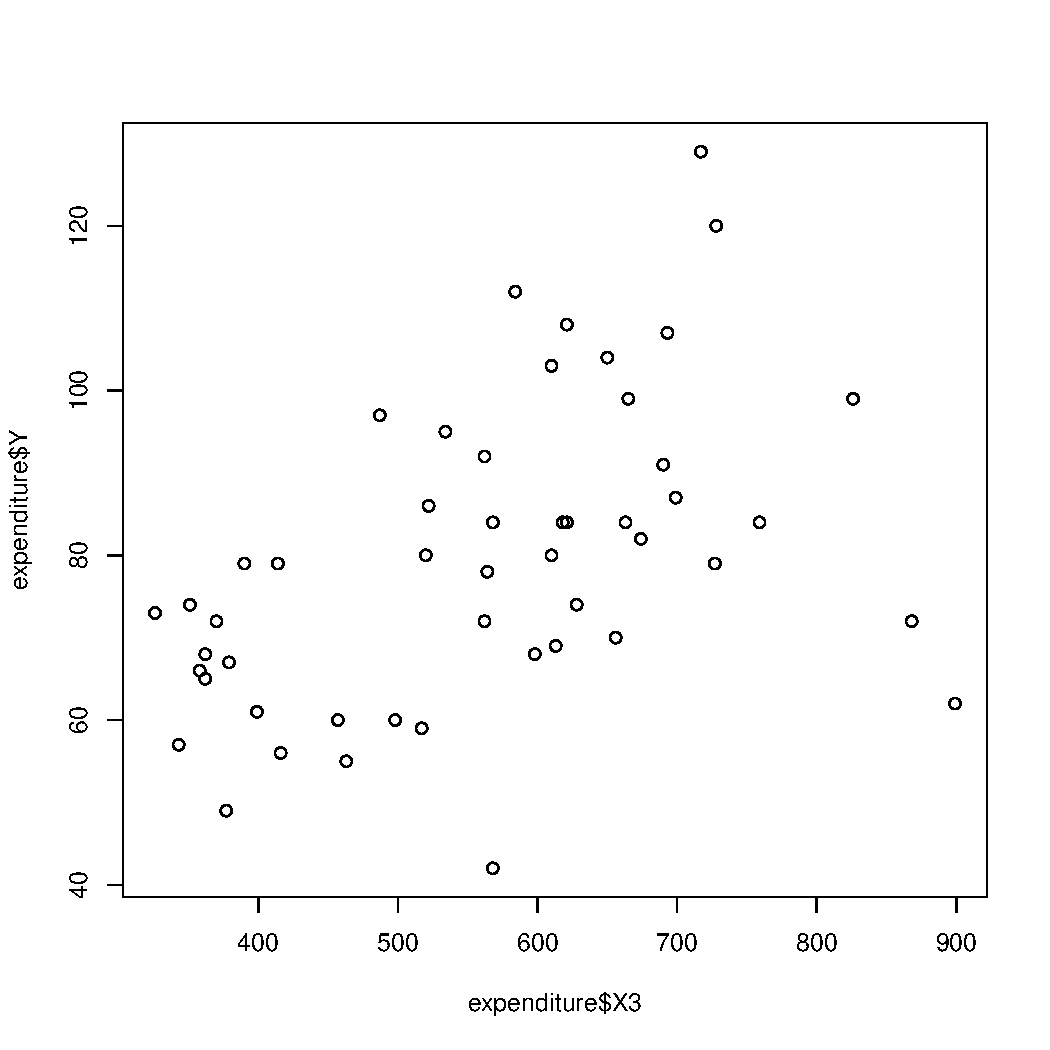
\includegraphics[width=.75\textwidth]{plot_Y_X3.pdf}
\end{figure}

\begin{figure}[hbtp!]\centering
	\caption{\footnotesize Relationship between X1 and Y.}
	\label{fig:plot_4}
	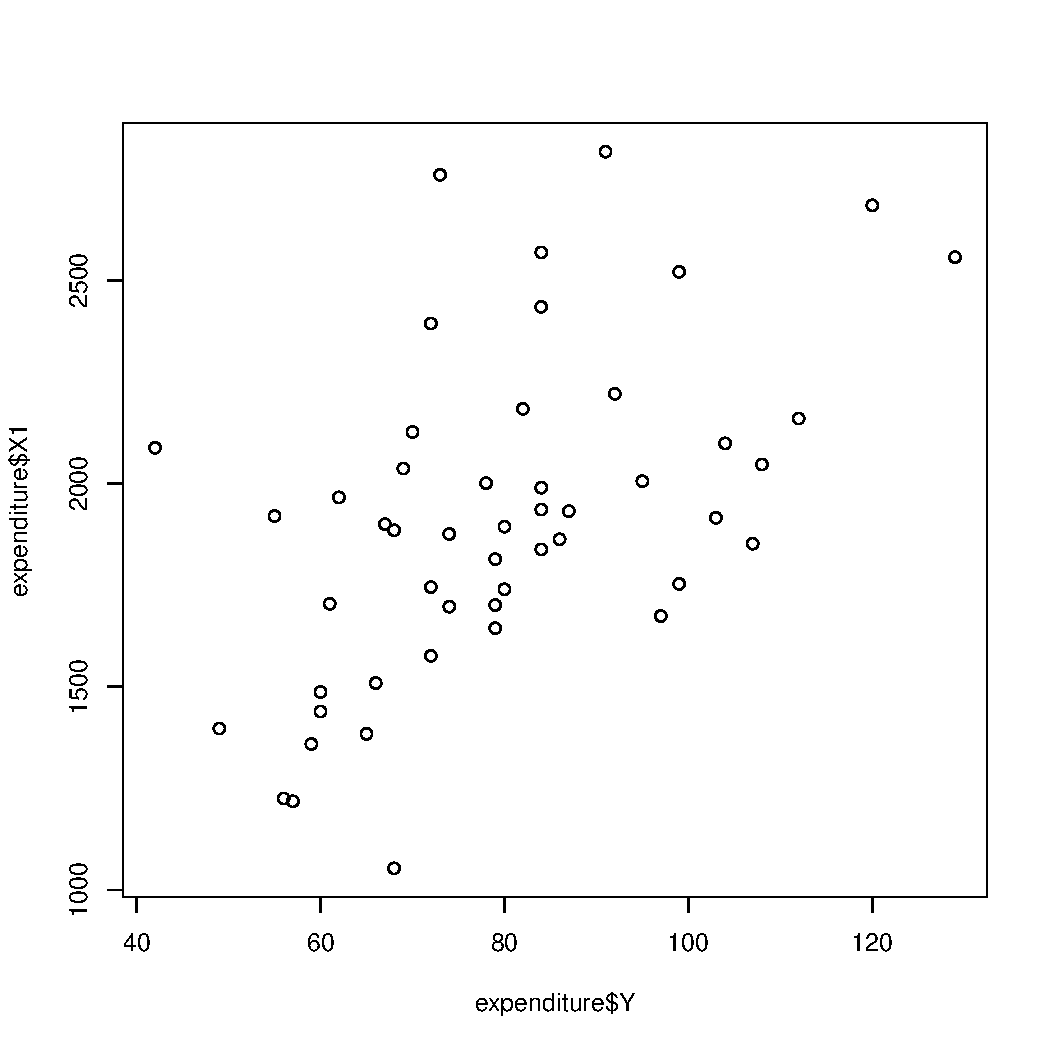
\includegraphics[width=.75\textwidth]{plot_X1_Y.pdf}
\end{figure}

\begin{figure}[hbtp!]\centering
	\caption{\footnotesize Relationship between X1 and X2.}
	\label{fig:plot_5}
	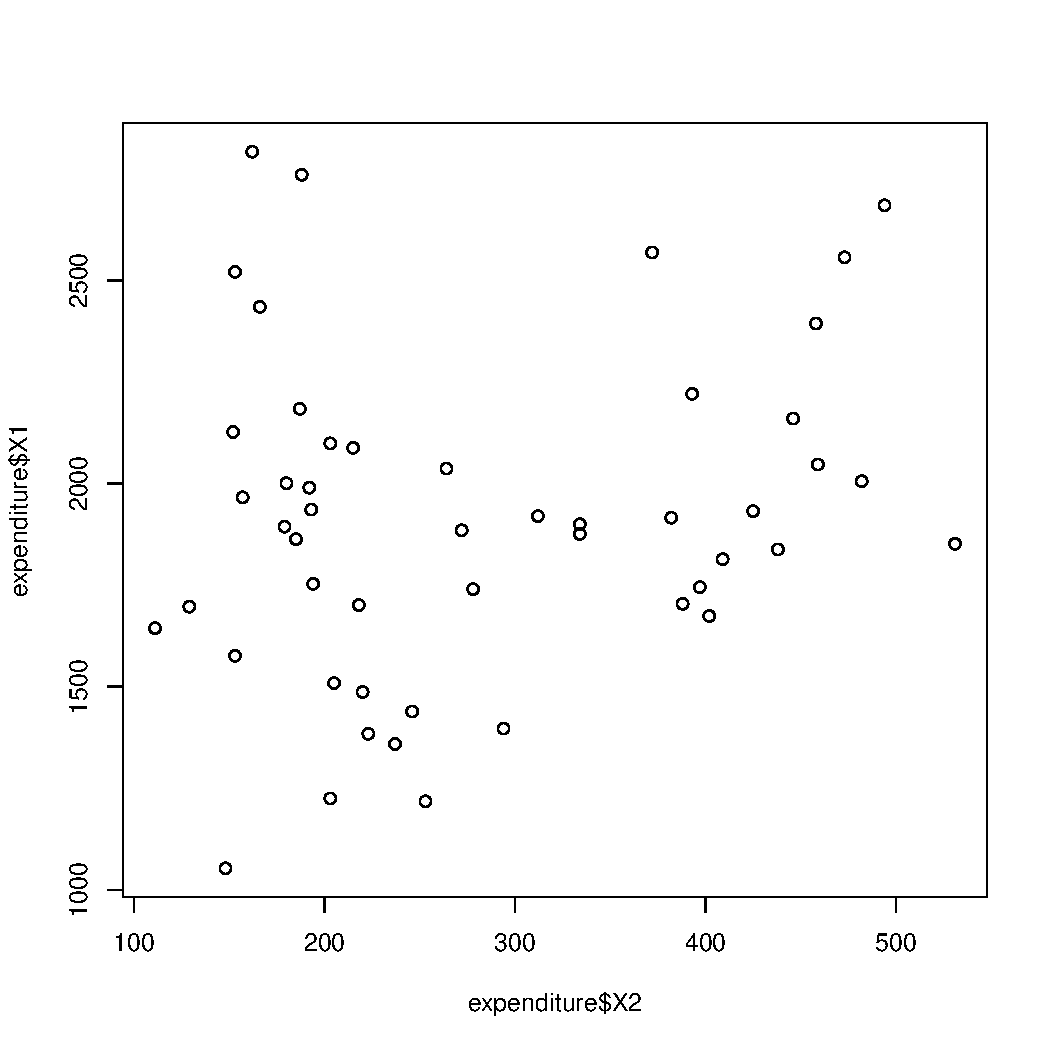
\includegraphics[width=.75\textwidth]{plot_X1_X2.pdf}
\end{figure}

\begin{figure}[hbtp!]\centering
	\caption{\footnotesize Relationship between X1 and X3.}
	\label{fig:plot_6}
	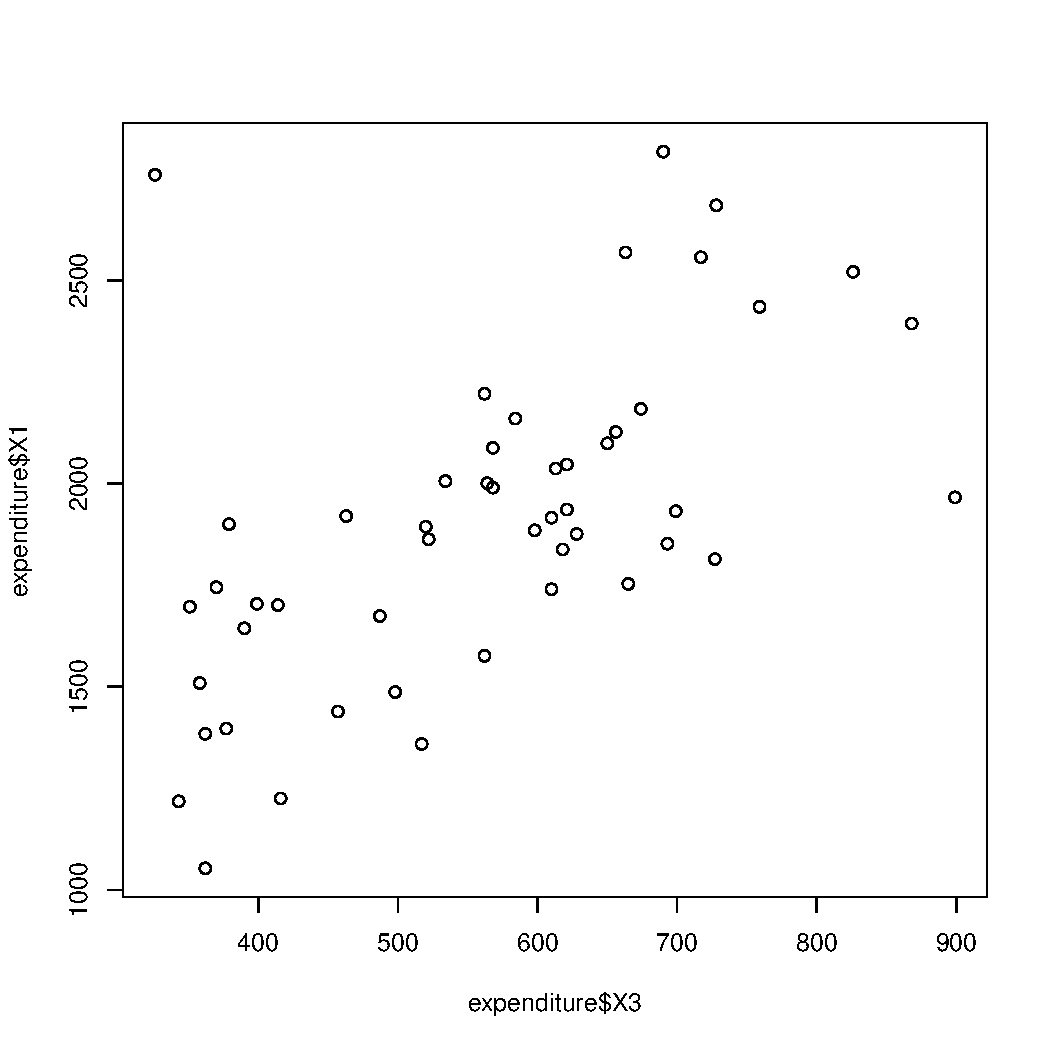
\includegraphics[width=.75\textwidth]{plot_X1_X3.pdf}
\end{figure}

\begin{figure}[hbtp!]\centering
	\caption{\footnotesize Relationship between X2 and Y.}
	\label{fig:plot_7}
	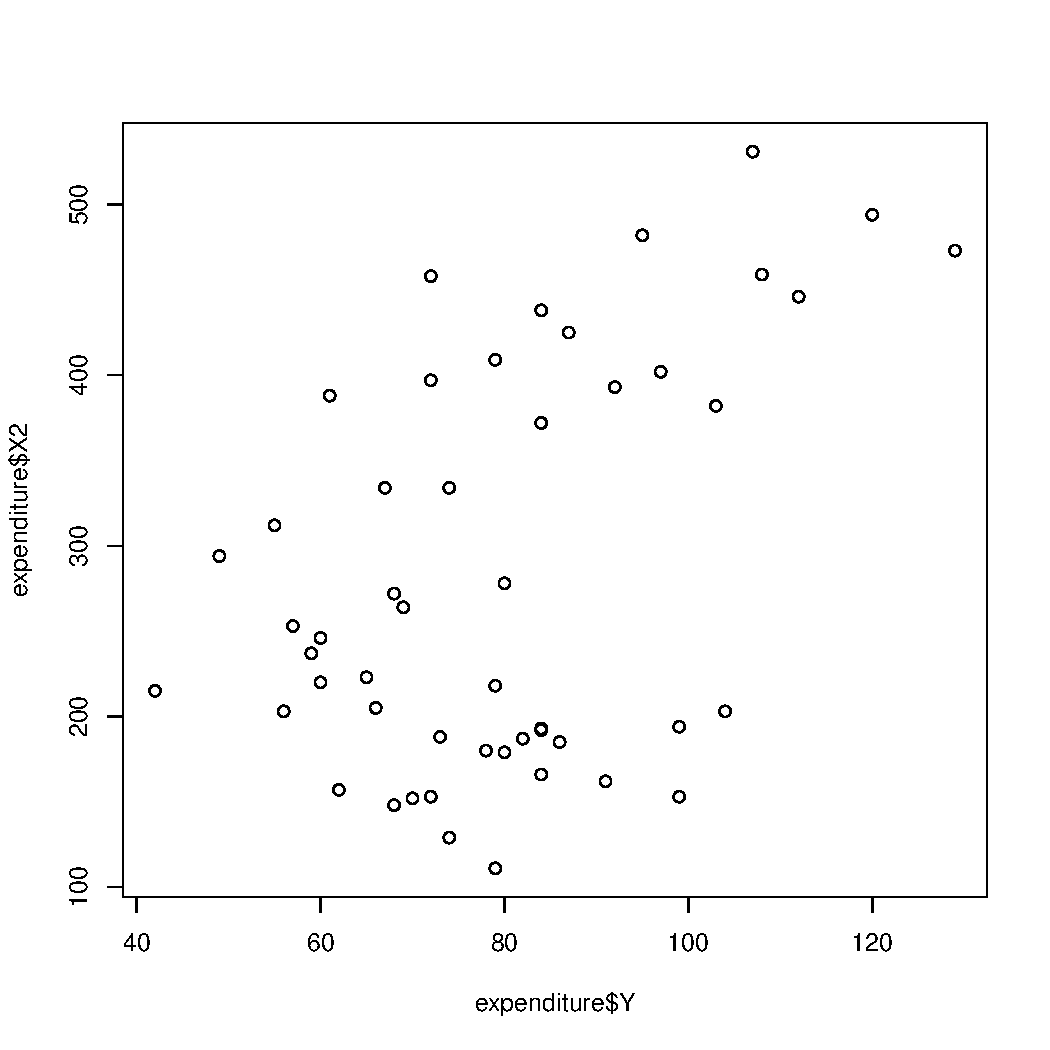
\includegraphics[width=.75\textwidth]{plot_X2_Y.pdf}
\end{figure}

\begin{figure}[hbtp!]\centering
	\caption{\footnotesize Relationship between X2 and X1.}
	\label{fig:plot_8}
	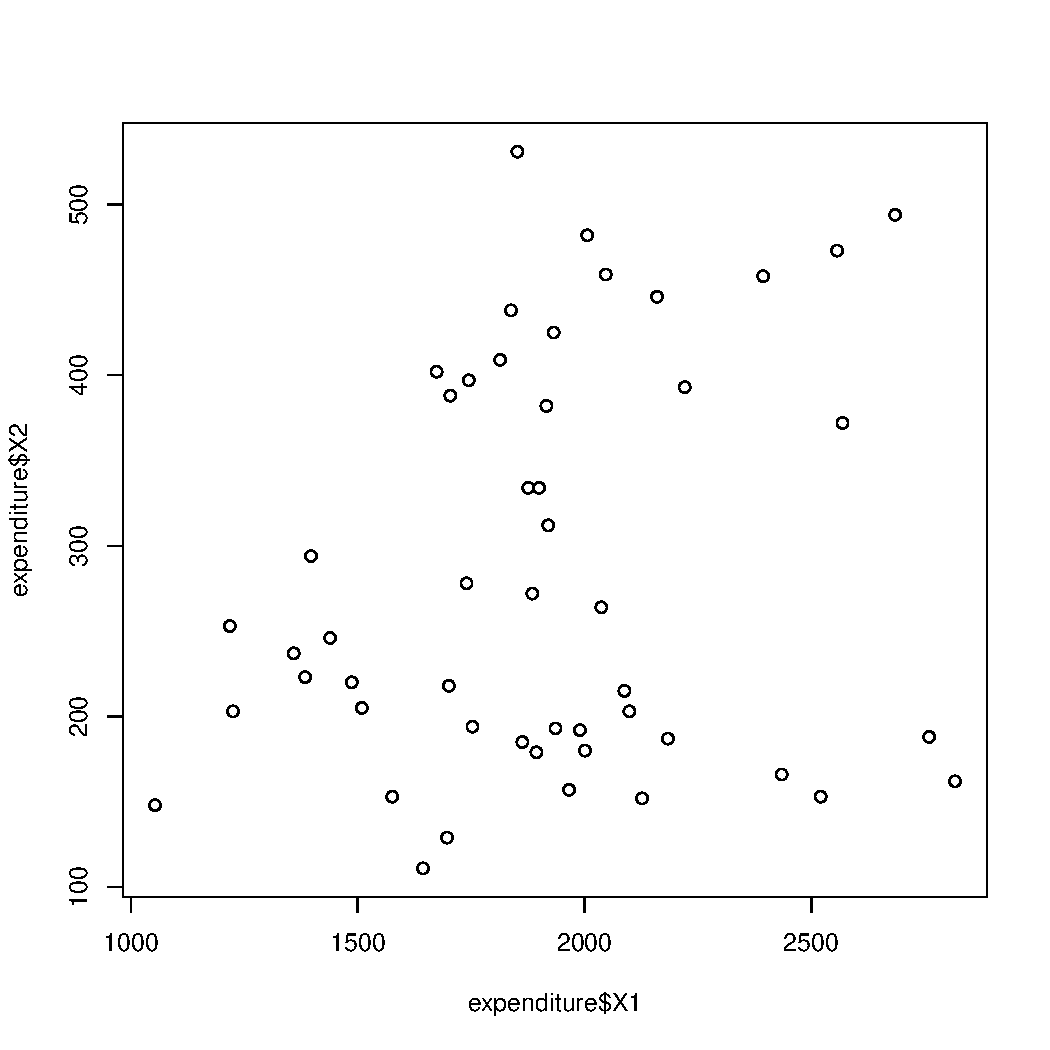
\includegraphics[width=.75\textwidth]{plot_X2_X1.pdf}
\end{figure}

\begin{figure}[hbtp!]\centering
	\caption{\footnotesize Relationship between X2 and X3.}
	\label{fig:plot_9}
	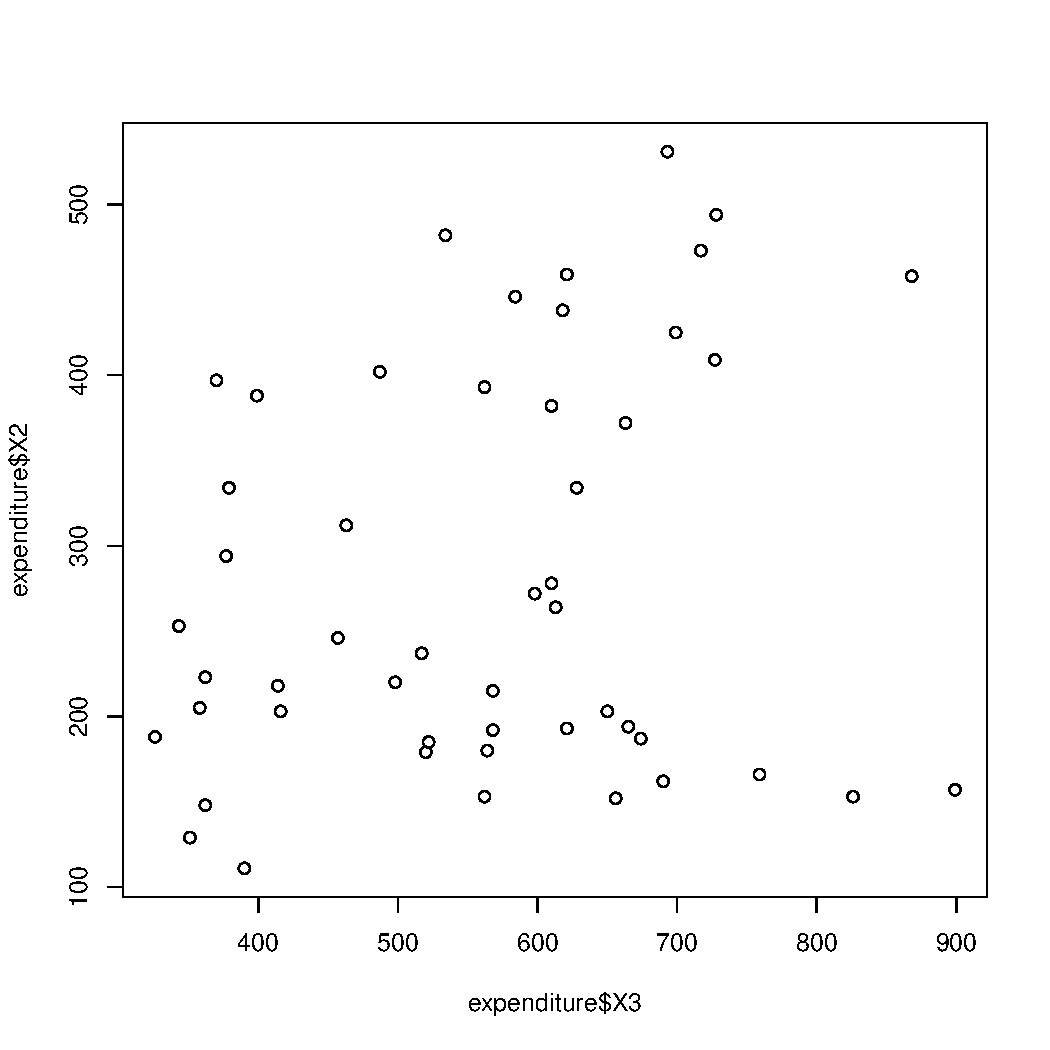
\includegraphics[width=.75\textwidth]{plot_X2_X3.pdf}
\end{figure}

\begin{figure}[hbtp!]\centering
	\caption{\footnotesize Relationship between X3 and Y.}
	\label{fig:plot_10}
	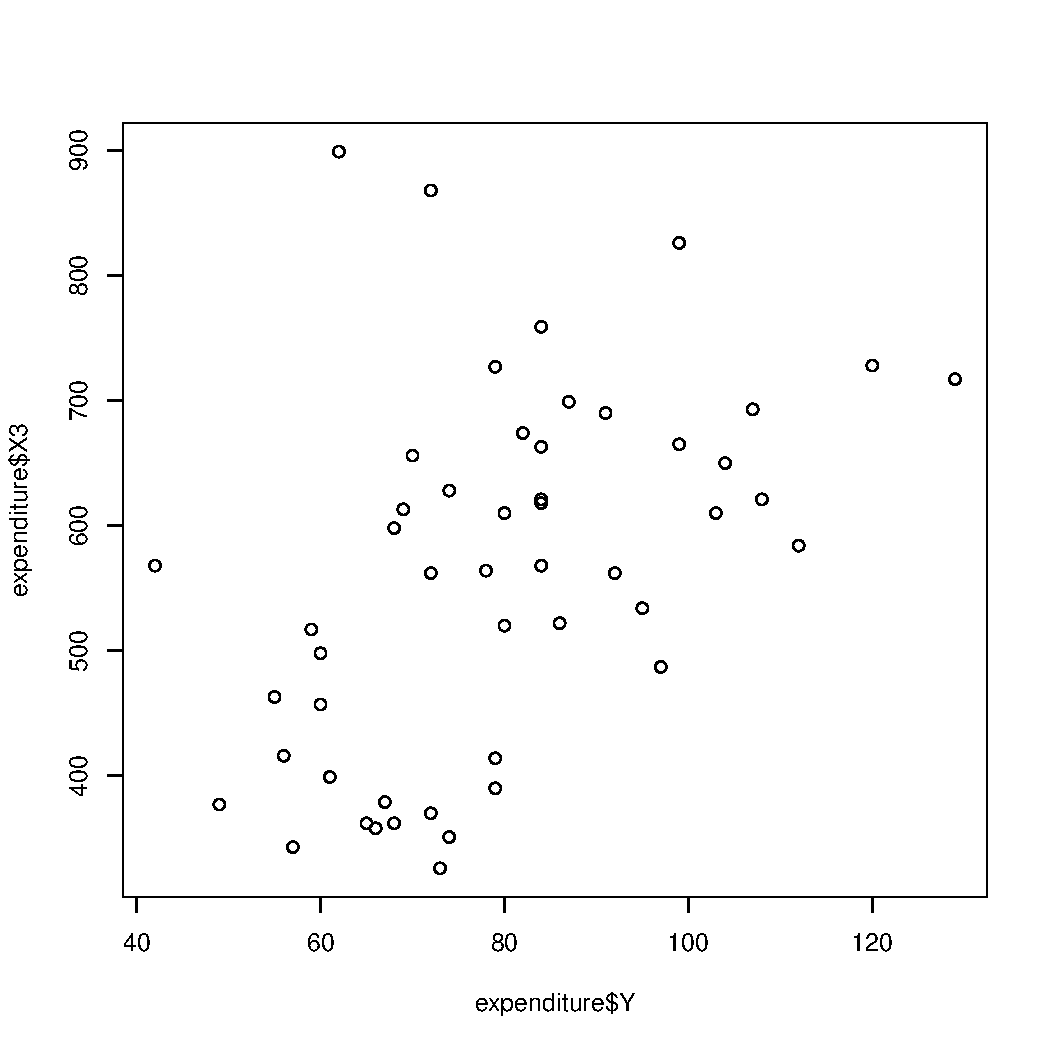
\includegraphics[width=.75\textwidth]{plot_X3_Y.pdf}
\end{figure}

\begin{figure}[hbtp!]\centering
	\caption{\footnotesize Relationship between X3 and X1.}
	\label{fig:plot_11}
	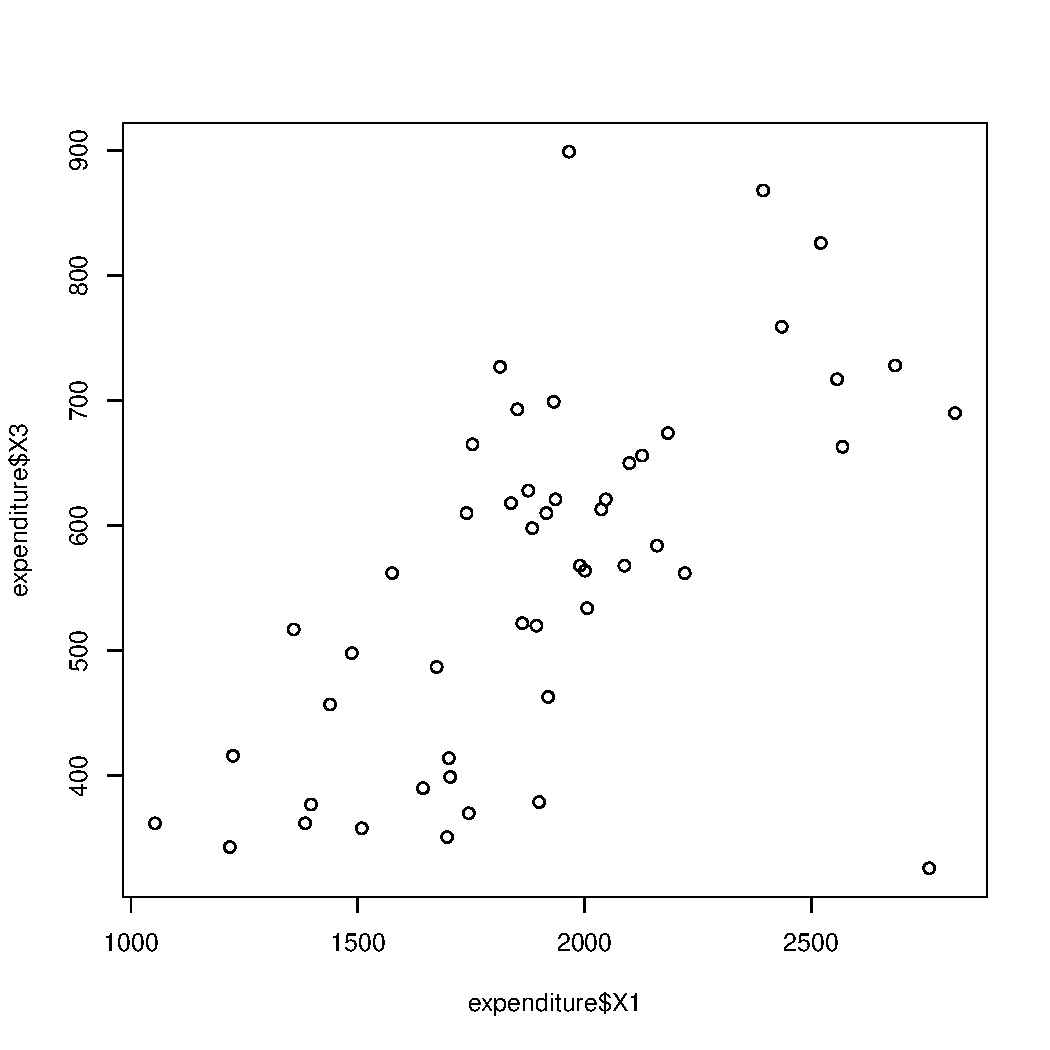
\includegraphics[width=.75\textwidth]{plot_X3_X1.pdf}
\end{figure}

\begin{figure}[hbtp!]\centering
	\caption{\footnotesize Relationship between X3 and X2.}
	\label{fig:plot_12}
	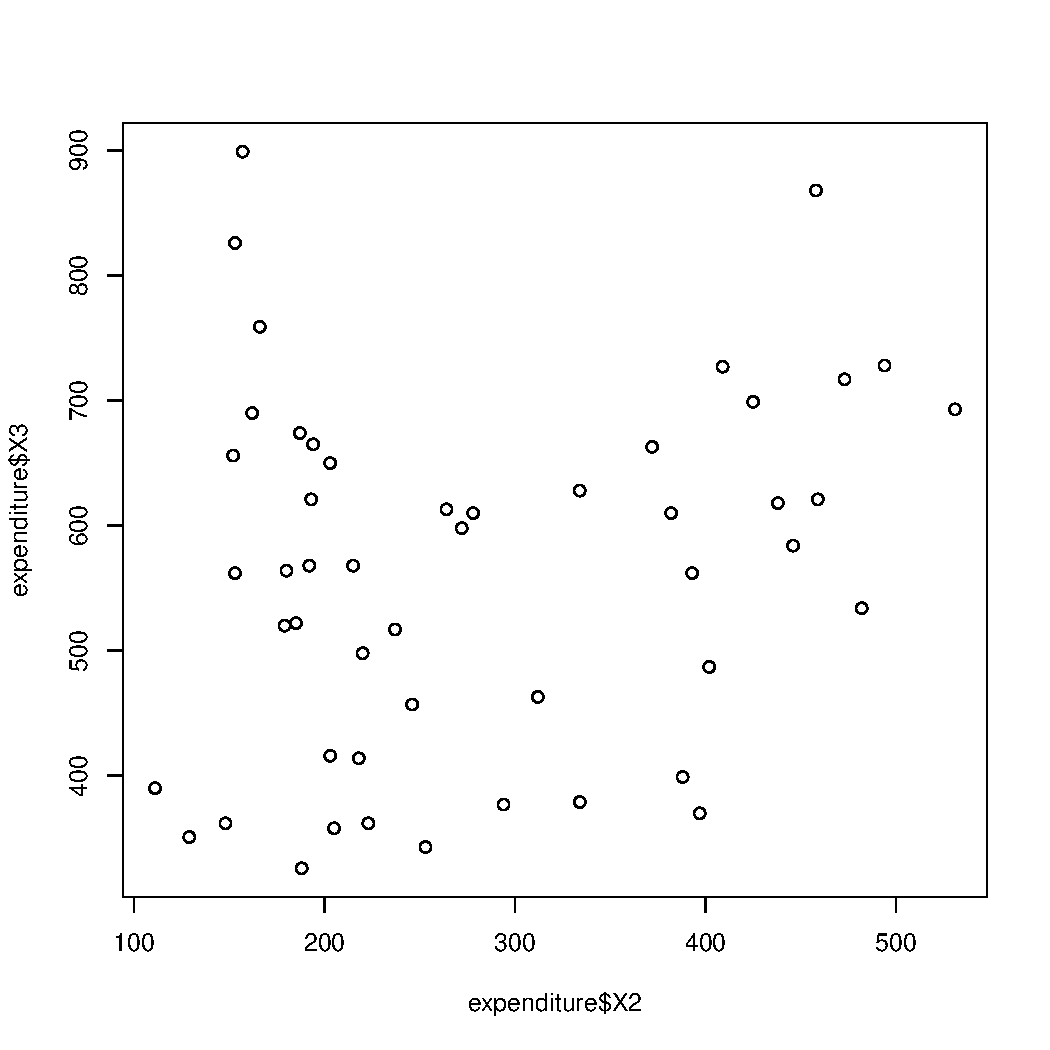
\includegraphics[width=.75\textwidth]{plot_X3_X2.pdf}
\end{figure}

\newpage
\item
Answer for Question 2.2\\

\noindent We begin by wrangling the data. We want to find the average per capita expenditure on housing assistance for each of the four regions.\\

\vspace{.5cm}
\lstinputlisting[language=R, firstline=189, lastline=197]{PS1_answers_LL.R}  
\vspace{.5cm}

\noindent We get the following:\\

\begin{verbatim}
> Region_1_Expend
[1] 79.44444
> Region_2_Expend
[1] 83.91667
> Region_3_Expend
[1] 69.1875
> Region_4_Expend
[1] 88.30769
\end{verbatim}
\vspace{.5cm}

\noindent Based on r's calculations, we see that on average Region 4 has the highest per capita expenditure on housing assistance, at 88.3 (assumed to be) USD. Let us use a boxplot to check the minimum and maximum points, as well as the median, and the first and third quartile for the four regions. The formula is as follows:\\

\vspace{.5cm}
\lstinputlisting[language=R, firstline=210, lastline=215]{PS1_answers_LL.R}  
\vspace{.5cm}

\begin{figure}[hbtp!]\centering
	\caption{\footnotesize Per capita expenditure on housing assistance by Regions.}
	\label{boxplot}
	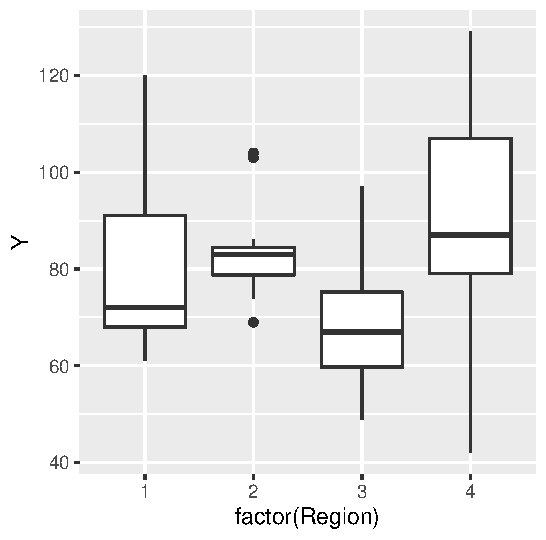
\includegraphics[width=.75\textwidth]{Rplot_Y_Region.pdf}
\end{figure}

\noindent Fig 13 shows that the boxplot for Region 4 (West), is observably higher than that of the other three regions, suggesting that it has on average, the highest per capita expenditure on housing assistance. Looking at the boxplots, 75 percent of the states in the West have a per capita expenditure on housing assistance of between 79 (assumed to be) and 129 USD. This is compared to between 68 and 120 for Region 1 (Northeast), between 60 and 98 for Region 3 (South), and between 79 and 85 for Region 2 (North Central). While Region 4 has on average, the highest per capita expenditure on housing assistance, it also has the longest boxplot and the longest whiskers, suggesting that the states within the region also have the largest disparity, or distribution, in the level of housing assistance expenditure per capita. Region 2 has the shortest boxplot and shortest whiskers, suggesting it has the smallest disparity in the level of housing assistance expenditure per capita. Region 2 is also interesting as it is the only region with outliers - it has three outliers.\\

\item
Answer for Question 2.3\\

\noindent We replot Y and X1, this time with more bells and whistles, using the below code:
\vspace{.5cm}
\lstinputlisting[language=R, firstline=234, lastline=235]{PS1_answers_LL.R}  
\vspace{.5cm}

\noindent The scatterplot below (Fig 14) shows a weak to medium positive, linear correlation between Y,  the per capita expenditure on shelters/housing assistance in state, and X1, the per capita personal income in state. This suggests there is a likelihood that with increasing personal capita personal income in state, there is increasing per capita expenditure on shelters/housing in state. There are a number of outliers in the data that need to be investigated.\\

\newpage
\begin{figure}[hbtp!]\centering
	\caption{\footnotesize Per capita expenditure on housing assistance by Regions.}
	\label{boxplot}
	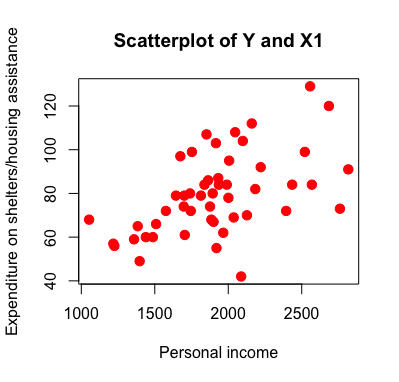
\includegraphics[width=.75\textwidth]{Rplot_Colour_Y_X1.png}
\end{figure}

\newpage
\noindent Next, we plot the above graph with a third variable, Region. The r code is reproduced as follows:
\vspace{.5cm}
\lstinputlisting[language=R, firstline=244, lastline=253]{PS1_answers_LL.R}  
\vspace{.5cm}

\noindent From the graph (Fig 15), we can observe more clearly the differences between the four regions. There are generally lower levels of per capita personal income and per capita expenditure on shelters/housing in the South. The Northeast tends to have higher levels of per capita personal income, but overall, per capita expenditure on shelters/housing is not particularly high, even though there are three states that are outliers in terms of shelter expenditure. The North Central lies somewhat in between the spread of the South and the Northeast. The points for the West look rather peculiar - with the majority of the data points concentrated between 1600 and 2100 on the x-axis. This seems to suggest there might be some form of basic income
# or minimum wage policy in many states in the West. In the West, unlike the other three regions, personal income levels do not seem to have a strong correlation with spending on housing/shelters.\\

\begin{figure}[hbtp!]\centering
	\caption{\footnotesize Per capita expenditure on housing assistance by Regions.}
	\label{boxplot}
	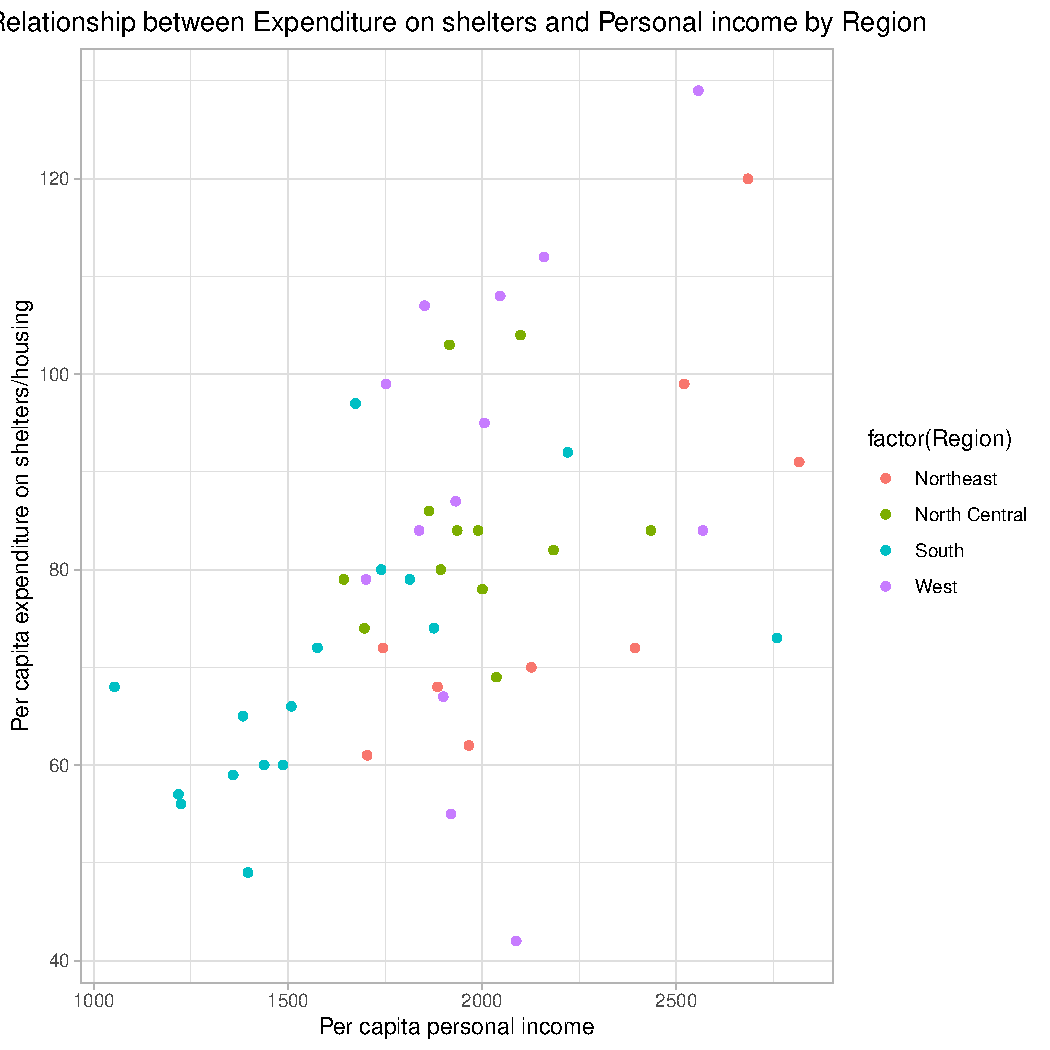
\includegraphics[width=.75\textwidth]{plot_3_variables.pdf}
\end{figure}

\end{itemize}

\end{document}